% questions.tex —— 1977 年·河南卷 · 题目内容片段（无答案）
% 由 tools/generate_projects.py 依来源总账自 1977/1977_数学真题_河南_试题.md 生成，勿手改（改源 MD 后重跑）


\gkpart{数学试题解}

\begin{gktip}
\textbf{来源说明}：本题面依据固定源 PDF《河南 1977 年高考数学试题解》第 1—5 页逐题转录，解答依据同一 PDF 第 1—6 页核对。固定源是题面与解答连续出现的扫描材料，而不是无答案试卷；正式题为第 1—10 题，末尾“参考题”的两题不计入题量。源 PDF 页面底部带有书籍页码 83—87，本文按 PDF 页序记录。
\end{gktip}

\begin{question}
\gkti{1}\textbf{（7 分）} 化简下式：

\nopagebreak[4]
\[
(1-c^2)^{-\frac12}
-\left\{[(1+c)(1-c)]^{\frac12}
+c^2[(1+c)(1-c)]^{-\frac12}\right\}.
\]

\end{question}
\begin{question}
\gkti{2}\textbf{（7 分）} 求

\nopagebreak[4]
\[
\frac{\lg3+\lg2}
{\frac14\lg16+\sqrt{(\lg1-\lg10)^2}+\frac12\lg0.09}
\]

的值。

\end{question}
\begin{question}
\gkti{3}\textbf{（7 分）} 求等式

\nopagebreak[4]
\[
5^{x^2-2x}=125
\]

中 $x$ 的值。

\end{question}
\begin{question}
\gkti{4}已知 $a\text{、}b\text{、}c$ 分别表示 $\triangle ABC$ 的角 $A\text{、}B\text{、}C$ 对边的长，求证：

\nopagebreak[4]
\[
a(\sin B-\sin C)+b(\sin C-\sin A)+c(\sin A-\sin B)=0.
\]

\Needspace{0.4\textheight}
\end{question}
\begin{question}
\gkti{5}\textbf{（8 分）} 如图，已知正方形 $ABCD$ 的边 $CD$ 上任意一点 $E$，延长 $BC$ 到 $F$，使 $CF=CE$，设 $BE$ 与 $DF$ 相交于 $G$，求证 $BG\perp DF$。

\begin{gktip}
原源 PDF 第 2 页附有正方形、延长线和交点 $G$ 的示意图；LaTeX 版按源图重绘。
\end{gktip}
\nopagebreak[4]
\begin{center}% 1977 年河南卷第五题：正方形 ABCD（A 左上、D 右上、B 左下、C 右下），
% E 在 DC 边上，F 在 BC 延长线上（CF=CE），BE 与 DF 交于 G（按源卷第 2 页布局）
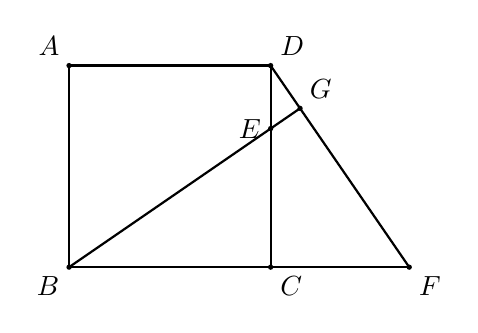
\begin{tikzpicture}[scale=0.8]
  \coordinate (A) at (0,3.2);
  \coordinate (D) at (3.2,3.2);
  \coordinate (C) at (3.2,0);
  \coordinate (B) at (0,0);
  \coordinate (E) at (3.2,2.2);
  \coordinate (F) at (5.4,0);
  \coordinate (G) at (3.667,2.521);
  \draw[thick] (A)--(D)--(C)--(B)--cycle;
  \draw[thick] (C)--(F);
  \draw[thick] (B)--(G);
  \draw[thick] (D)--(F);
  \fill (A) circle (1.2pt) node[above left] {$A$};
  \fill (D) circle (1.2pt) node[above right] {$D$};
  \fill (C) circle (1.2pt) node[below right] {$C$};
  \fill (B) circle (1.2pt) node[below left] {$B$};
  \fill (E) circle (1.2pt) node[left] {$E$};
  \fill (F) circle (1.2pt) node[below right] {$F$};
  \fill (G) circle (1.2pt) node[above right] {$G$};
\end{tikzpicture}
\end{center}
\nopagebreak[4]
\end{question}
\begin{question}
\gkti{6}\textbf{（10 分）} 求证：

\nopagebreak[4]
\[
\operatorname{tg}^2\alpha-\operatorname{ctg}^2\alpha
=-\frac{2\sin4\alpha}{\sin^3 2\alpha}.
\]

\Needspace{0.4\textheight}
\end{question}
\begin{question}
\gkti{7}\textbf{（10 分）} 已知长方体的对角线长为 $L$，它与底面所成的角为 $\alpha$，底面两条对角线的夹角为 $\beta$，求长方体的体积。

\begin{gktip}
原源 PDF 第 3 页附有长方体和底面对角线夹角示意图；LaTeX 版按源图重绘。
\end{gktip}
\nopagebreak[4]
\begin{center}% 1977 年河南卷第七题：长方体 ABCD-A1B1C1D1（顶面 A1B1C1D1），
% 体对角线 A1C（虚线）与底面所成角 α 标在 C 处，底面对角线 AC、BD 夹角 β 标在中心（按源卷第 3 页布局）
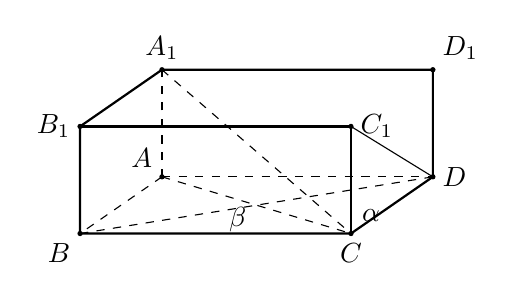
\begin{tikzpicture}[scale=0.8]
  \coordinate (B) at (0,0.8);
  \coordinate (C) at (4.3,0.8);
  \coordinate (D) at (5.6,1.7);
  \coordinate (A) at (1.3,1.7);
  \coordinate (B1) at (0,2.5);
  \coordinate (C1) at (4.3,2.5);
  \coordinate (D1) at (5.6,3.4);
  \coordinate (A1) at (1.3,3.4);
  \draw[thick] (B)--(C)--(D)--(D1)--(A1)--(B1)--cycle;
  \draw[thick] (B)--(B1);
  \draw[thick] (C)--(C1);
  \draw[thick] (A1)--(D1);
  \draw[thick] (B1)--(C1);
  \draw[thin] (C1)--(D);
  \draw[dashed] (A)--(B);
  \draw[dashed] (A)--(D);
  \draw[dashed] (A)--(A1);
  \draw[dashed] (A)--(C);
  \draw[dashed] (B)--(D);
  \draw[dashed] (A1)--(C);
  \fill (A) circle (1.2pt) node[above left] {$A$};
  \fill (B) circle (1.2pt) node[below left] {$B$};
  \fill (C) circle (1.2pt) node[below] {$C$};
  \fill (D) circle (1.2pt) node[right] {$D$};
  \fill (A1) circle (1.2pt) node[above] {$A_1$};
  \fill (B1) circle (1.2pt) node[left] {$B_1$};
  \fill (C1) circle (1.2pt) node[right] {$C_1$};
  \fill (D1) circle (1.2pt) node[above right] {$D_1$};
  \node at (4.62,1.08) {$\alpha$};
  \node at (2.5,1.02) {$\beta$};
\end{tikzpicture}
\end{center}
\nopagebreak[4]
\end{question}
\begin{question}
\gkti{8}\textbf{（14 分）} 某工厂科研小组，对一项生产工艺过程总结出产量指标函数和消耗函数为：

\nopagebreak[4]
\[
f_1(x)=a_1x^2+\frac12x+c
\qquad\text{\text{和}}\qquad
f_2(x)=a_2x^2+bx+\frac54\quad\text{（※）}
\]

\Needspace{5\baselineskip}
且知

\nopagebreak[4]
\[
f_1(-1)=f_2(-1)=f_1(3)=f_2(3)=2.
\]

（1） 分别求出产量指标函数 $f_1(x)$ 和消耗函数 $f_2(x)$ 的具体表达式；

（2） 问因素 $x$ 取何值时，$f_1(x)$ 和 $f_2(x)$ 有最大值或最小值？最大值或最小值各是多少？

（3） 画出所求出函数的略图。

\begin{gktip}
\textbf{源注}：原题中 $a_1=a_2=a$，问题无解；源解答注明“酌情把 $f_1(x)$ 和 $f_2(x)$ 中的二次项系数分别改为 $a_1$ 和 $a_2$”。本文按该源注所对应的可解题面转录，并保留这一更正说明。
\end{gktip}

\end{question}
\begin{question}
\gkti{9}\textbf{（14 分）} 已知过点 $P(0,3\sqrt2)$ 且斜率为 $k$ 的直线与圆心在原点、半径为 $3$ 的圆相交于 $M\text{、}N$ 两点。

（1） 求 $M\text{、}N$ 的坐标；

（2） 问当 $M\text{、}N$ 两点重合时，$k$ 为何值？过 $P$ 点的直线与圆的位置关系如何？这样的直线有几条？它们的夹角是多大？

\begin{gktip}
\textbf{题号说明}：固定源第 4—5 页在第九题中直接印作“（1）”和“（3）”，未见“（2）”题干。本库题库规范要求小问连续编号，故将源卷“（3）”重排为“（2）”，未增删任何题干内容。
\end{gktip}

\end{question}
\begin{question}
\gkti{10}某电管所为实现农业现代化，加强电力网的建设，沿着一条通往农村的新公路栽电杆。已知一辆汽车每次从电管所运 3 根电线杆，相邻两根电线杆相距 50 米，汽车往返的总路程是 35.5 公里，最后一根电线杆与电管所相距 2450 米。

（1） 第一根电线杆与电管所相距多少？

（2） 共栽了多少根电线杆？

\Needspace{5\baselineskip}
\textbf{参考题 1．（20 分）} 已知

\nopagebreak[4]
\[
x+x^{-1}=2\cos\theta,
\]

\Needspace{5\baselineskip}
求证

\nopagebreak[4]
\[
x^n+x^{-n}=2\cos n\theta.
\]

\textbf{参考题 2．}

\Needspace{5\baselineskip}
（1） 设

\nopagebreak[4]
\[
y=\operatorname{Ln}\left(x+\sqrt{x^2-a^2}\right),
\]

求 $y$ 的导数 $y'$。

\Needspace{5\baselineskip}
（2） 求

\nopagebreak[4]
\[
\int_0^{2p}\sqrt{2px}\,dx
\]

的值。

\end{question}